\documentclass{article}
\usepackage{graphicx} % Required for inserting images
\usepackage[a4paper, margin=1in]{geometry}
\usepackage[a4paper, left=1.5cm, right=1.5cm, top=1cm, bottom=2cm]{geometry}
\usepackage{hyperref}


\title{Introducción a Packet Tracer}
\author{Octavio Pendino}
\date{August 2024}

\begin{document}

\maketitle

\section{Packet Tracer}
Cisco Packet Tracer es un programa de simulación de redes desarrollado por Cisco Systems. Este software se utiliza principalmente para crear y simular redes informáticas, permitiendo a los usuarios diseñar, configurar y poner en funcionamiento redes virtuales. También es una herramienta de aprendizaje ampliamente utilizada en la capacitación de redes y la preparación para exámenes de certificación de Cisco, como CCNA y CCNP. Los usuarios pueden experimentar con diferentes configuraciones de red y escenarios sin la necesidad de hardware físico.

    Packet Tracer ofrece distintas herramientas para diseñar, configurar y probar redes virtuales. Entre las principales se encuentran:
    \begin{itemize}
        \item Dispositivos de Red como Routers, Switches, Hubs.
        \item Dispositivos Finales como PCs, Laptops, Servidores, etc.
        \item Cables para conectar dispositivos entre sí, cables de consola, etc.
        \item Componentes para simulaciones IoT.
        \item Herramientas de configuración como CLI para configurar dispositivos mediante comandos, configurador de IP, etc.
        \item Herramientas de prueba y diagnóstico.
        \item Modo peer-to-peer que permite múltiples usuarios y la construcción de una red simulada de forma colaborativa.
    \end{itemize}

\subsection{Espacios de trabajo}
     Packet Tracer tiene dos espacios de trabajo: el lógico y el físico. 
     \begin{enumerate}
         \item El espacio de trabajo lógico permite a los usuarios construir topologías de red lógicas colocando, conectando y agrupando dispositivos de red de forma virtual. En este espacio, la red se representa de manera abstracta, mostrando cómo los dispositivos están conectados lógicamente entre sí
         \item El espacio de trabajo físico proporciona una dimensión física gráfica de la red lógica, dando un sentido de escala y ubicación en la forma en que los dispositivos se verían en un entorno real.Permite ver y gestionar la disposición física de los dispositivos, así como su cableado y conectividad. 
     \end{enumerate}
\subsection{Modos de operación}
Proporciona dos modos de funcionamiento para visualizar el comportamiento de una red: en tiempo real y modo de simulación.
\begin{enumerate}
         \item El Modo en Tiempo Real es el modo predeterminado en Packet Tracer. En este modo la red se comporta como lo haría en la realidad, los eventos se simulan exactamente como los ejecutarían los dispositivos reales. Las cosas suceden casi inmediatamente y podemos hacer pruebas en tiempo real.
         \item El modo de simulación es un modo especial en el que se puede observar cómo viajan los paquetes entre los dispositivos. Éste modo permite ver a un alto nivel de detalle lo que pasa en la red y controlar el nivel de detalle que se desea ver. Podemos controlar los intervalos de tiempo, la transferencia de datos y el funcionamiento interno de la red. 
     \end{enumerate}
\section{Dispositivos finales}
Los dispositivos finales (End Devices) o hosts son los dispositivos que se encuentran al final de una red y que interactúan directamente con los usuarios o aplicaciones. Estos dispositivos son fundamentales en una red porque son los puntos donde se inicia o se recibe el tráfico de red, y son utilizados por los usuarios para acceder a servicios y recursos de la red. Estos dispositivos forman la interfaz entre los usuarios y la red de comunicación subyacente. Un dispositivo host es el origen o el destino de un mensaje transmitido a través de la red. Para distinguir un host de otro, cada host en la red se identifica por una dirección. Cuando un host inicia la comunicación, utiliza la dirección del host de destino para especificar a dónde se debe enviar el mensaje. En las redes modernas, un hosts pueden actuar como un cliente, un servidor o ambos. El software instalado en el host determina qué función tiene en la red. Packet Tracer ofrece distintos dispositivos finales para conectarlos entre sí, configurarlos y realizar distintas simulaciones. Durante la cursada vamos a ver principalmente los siguientes:
\begin{itemize}
    \item PCs y Laptops, podemos asignarles direcciones IP, configurar su gateway, y usar herramientas como Ping y Traceroute para pruebas de conectividad. Tambien permite conectar dispositivos externos como microfonos y auriculares.
    \item Servidores, en los cuales podemos configurar los servidores para que ofrezcan diferentes servicios, EMAIL, HTTP, FTP, DNS, etc.
    \item Impresoras, podemos asignarles direcciones IP y configurar la red para que otros dispositivos puedan enviar trabajos de impresión.
\end{itemize}
\begin{figure}[h]
  \centering
  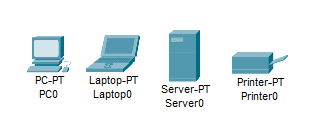
\includegraphics[width=0.5\textwidth]{Dispositivos finales.png}
  \caption{Dispositivos finales}
\end{figure}
A su vez, los dispositivos finales en Packet Tracer (PC, Servidor, Impresora y Teléfono IP) cuentan con un slot para módulos de diferentes interfaces que se pueden intercambiar para adecuarlos a la topología que queremos simular.

Los módulos PT-HOST-NM-1W y Linksys-WMP300 son interfaces inalámbricas de 2.4 GHz.

Los módulos PT-HOST-NM-1CE (Ethernet), PT-HOST-NM-1CFE (Fast Ethernet 10/100BaseTX) y PT-HOST-NM-1CGE (Gigabit Ethernet) son interfaces Ethernet para cobre.

Los módulos PT-HOST-NM-1FFE (Fast Ethernet 100BaseFX) y PT-HOST-NM-1FGE (Gigabit Ethernet) son interfaces Ethernet para Fibra Óptica.

El módulo PT-HOST-NM-1AM es la interface de un Módem.

En la PC podemos utilizar todos los módulos, en el Server y la Impresora no contamos con el módulo para Modem.
\section{Dispositivos de red}
Los dispositivos de red / dispositivos intermediarios son componentes fundamentales que permiten la interconexión, administración y control del tráfico de datos dentro de una red. En Packet Tracer simulan el hardware real que se usa en redes informáticas para tareas como el enrutamiento, conmutación, acceso a Internet, y más. Proporcionan conectividad y operan detrás de escena para asegurar que los datos fluyan a través de la red, conectan los hosts individuales a la red y pueden conectar varias redes individuales para formar una internetwork. Estos dispositivos utilizan la dirección host de destino, conjuntamente con información sobre las interconexiones de la red, para determinar la ruta que deben tomar los mensajes a través de la red. Los dispositivos de red con los que vamos a trabajar son:
\begin{itemize}
    \item Routers, son dispositivos que determinan la mejor ruta para enviar paquetes de datos entre diferentes redes. Son cruciales para conectar múltiples redes y gestionar el tráfico entre ellas. Packet Tracer ofrece una gran cantidad de routers para trabajar, entre ellos tenemos: 

    - 4331 y 4321 con IOS-XE versión 16, son los modelos vigentes a la fecha, con disponibilidad para interfaces GigabitEthernet de cobre y fibra de capa 3 e interfaces GigabitEthernet de capa 2.

    -  2911 y 2901 con IOS versión 15, son modelos no muy recientes pero tienen disponibilidad para interfaces GigabitEthernet de cobre y fibra de capa 3, interfaces FastEthernet de capa 2 e interfaces seriales.
    
    Los routers en Packet Tracer permiten la adición y eliminación de módulos para personalizar las capacidades del dispositivo. Algunos módulos son: HWIC-2T (Proporciona dos puertos seriales para conexiones WAN), HWIC-4ESW (Añade 4 puertos de switch al router), NM-1FE-TX (Añade un puerto Fast Ethernet al router), etc. Los módulos disponibles dependerán del router que se utilice.

    Los routers tienen varias interfaces que se pueden usar para conectarse a diferentes tipos de redes. Las interfaces son los puntos de conexión físicos o virtuales a través de los cuales un router puede enviar y recibir datos hacia y desde otras redes o dispositivos. Cada interfaz se asocia con una red específica y tiene su propia dirección IP, que permite al router comunicarse con dispositivos en esa red. Entre las interfaces, se encuentran: Fast Ethernet (interfaces con una velocidad de 100 Mbps), Gigabit Ethernet (interfaces más rápidas con una velocidad de 1 Gbps), Serial (interfaces utilizadas para conexiones WAN), etc. Al igual que con los módulos, las interfaces disponibles dependerán del router con el que se esté trabajando.

    \item Switches, son dispositivos que interconectan múltiples dispositivos dentro de una misma red local (LAN), gestionan el tráfico de datos entre ellos y envían los datos solo al dispositivo destinatario correcto, lo que optimiza el uso de la red. Permite a los dispositivos conectados compartir información y comunicarse entre sí. Un switch no proporciona acceso a Internet, su objetivo es crear una red local donde sea posible compartir recursos fácilmente entre los dispositivos conectados. Packet Tracer ofrece distintos switches:
    
    - 2960, con IOS versión 15, Switch de capa 2 con 24 puertos FastEthernet e interfaces uplink GigabitEthernet de cobre.

    - 3560, con IOS versión 12, Switch de capa 3 con 24 puertos FastEthernet PoE e interfaces uplink GigabitEthernet de cobre.

    - 3650, con IOS-XE versión 16, Switch de capa 3 con 24 puertos GigabitEthernet PoE e interfaces uplink GigabitEthernet de cobre o fibra.

    \item Hubs, son dispositivos de red básicos que permiten la interconexión de múltiples dispositivos dentro de una red local (LAN). A diferencia de los switches, los hubs no son "inteligentes" y no pueden identificar el destino específico de los datos que reciben. En lugar de enviar los datos solo al dispositivo de destino, un hub simplemente retransmite los datos recibidos a todos los puertos conectados, lo que puede generar tráfico innecesario en la red.
\end{itemize}
\begin{figure}[h]
  \centering
  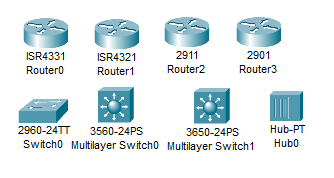
\includegraphics[width=0.5\textwidth]{dispositivos de red.png}
  \caption{Dispositivos de red}
\end{figure}
\subsection{Firmware}
El firmware es un tipo de software que está incrustado en un dispositivo de hardware para controlar su funcionamiento básico. A diferencia del software de aplicación que los usuarios pueden instalar o desinstalar, el firmware está programado en el hardware desde el momento de su fabricación y es esencial para que el dispositivo funcione correctamente.

El firmware en routers y switches de Cisco, es el software que proporciona las instrucciones básicas para que el dispositivo funcione y administre la red. Este firmware incluye el sistema operativo del dispositivo, que en el caso de los dispositivos Cisco suele ser Cisco IOS (Internetwork Operating System).

En Cisco Packet Tracer se puede simular la configuración y el uso del firmware de los routers y switches como si se estuviera utilizando un dispositivo físico de Cisco. Para dispositivos intermedios, como enrutadores y conmutadores, hay dos métodos de configuración disponibles.Los dispositivos se pueden configurar o revisar a través de una pestaña de Configuración (una interfaz GUI), o una interfaz de línea de comandos (CLI). La interfaz gráfica proporciona una forma de rápida de completar el espacio en blanco para hacer las configuraciones básicas y muestra los comandos de la CLI equivalentes que harían lo mismo si usara la interfaz de línea de comandos. Por otro lado, la interfaz CLI requiere conocimiento de la configuración del dispositivo.
\section{Cableado}
Como vimos hasta ahora, Cisco Packet Tracer ofrece una gran cantidad de dispositivos para diseñar y simular redes de computadoras. Para conectar los diferentes dispositivos que conforman la red, cuenta con diferentes medios de transmisión (cables y conectores), los cuales son fundamentales para  para conectar dispositivos de red y permitir la comunicación entre ellos. Los cables actúan como medios físicos a través de los cuales se transmiten señales (eléctricas, ópticas o inalámbricas) entre dispositivos de red, permitiendo la comunicación entre computadoras, switches, routers y otros dispositivos. Packet Tracer nos ofrece los siguientes cables para realizar nuestras conexiones:
\begin{itemize}
    \item Cable que selecciona automaticamente el tipo de conexión, es útil cuando desconocemos el tipo de cable que debemos usar para establecer la conexión. 
    \item Cable de consola,  proporciona la conexión entre un PC y un equipo de red CISCO, esto para poder realizar las configuraciones necesarias de este y así poder hacer que este sea utilizable. Dentro de los equipos de red que podemos configurar con este cable se encuentran routers, switches, access point, equipos de VoIP, entre otros.
    \item Cable de Cobre, es el más utilizado para interconectar todos los dispositivos que conforman una red LAN, siendo el encargado de transportar todos los datos informáticos. El más sencillo y común es el tipo UTP que consiste en hilos de cobre. Se realizan dos tipos de conexiones con cable ethernet de cobre utilizando el estándar EIA/TIA 568-A y EIA/TIA 568-B: 

        Cable de cobre directo, ambos extremos terminan con el mismo estándar, es decir, ambos entremos con el estándar EIA/TIA 568-A o ambos extremos con el estándar EIA/TIA 568-B. Sirven para conectar equipos que NO trabajen en la misma capa o que NO sean equipos iguales, como una computadora a un switch o un router a un switch.

        Cable de cobre cruzado, ambos extremos terminan con un estándar diferente, es decir, en un extremo usa el estándar EIA/TIA 568-A y al otro extremo usa el estándar EIA/TIA 568-B. Sirven para conectar equipos que trabajen en la misma capa ó que sean equipos iguales, como conectar una computadora a otra computadora o un switch a otro switch.

    \item Cable de Fibra Óptica, utilizan señales de luz para transmitir datos, lo que permite mayor velocidad y distancias más largas. Solo funcionan para dispositivos con puertos de fibra. Actualmente es muy utilizado para interconectar dispositivos de redes como Switches y Routers. Es ideal para conexiones en una red donde se requiere alta velocidad y baja latencia.

    \item Cable de Telefono, las conexiones de línea telefónica sólo puede hacerse entre dispositivos con puerto de módem. Se utiliza para la conexión de dispositivos como módems o teléfonos.

    \item Cable Coaxial, conecta dispositivos utilizando la tecnología más antigua basada en cables coaxiales, como en redes antiguas o algunas conexiones de TV. Es el tipo de cable utilizado en topologías de red antiguas. Hoy en día se utiliza en transmisiones de televisión por cable.

    \item Cable Serial, se utilizan para conexiones WAN (Wide Area Network) entre routers. Estos cables permiten la comunicación punto a punto entre routers, simulando enlaces de larga distancia que se utilizan en redes más grandes que abarcan múltiples ubicaciones. Hay 2 extremos en un cable serial: 

    DCE (Data Communication Equipment), es utilizado para conectar un router a otro router. En una conexión DCE-DTE el router con el cable DCE es responsable de establecer el ritmo de transmisión de datos en la conexión serial. Proporciona la señal de reloj que sincroniza la comunicación entre ambos dispositivos.

    DTE (Data Terminal Equipment), se utiliza para conectar el otro extremo de la conexión serial a un segundo router. Es el dispositivo que recibe la señal de reloj generada por el DCE. Sigue el ritmo establecido por el DCE para mantener la sincronización durante la transmisión de datos.

    \item Cable Octal, es un cable de consola especial que tiene un extremo que se conecta a un puerto serie en un servidor terminal o router, y el otro extremo se divide en múltiples conexiones de consola, típicamente ocho, que se conectan a diferentes dispositivos de red. Se utiliza para administrar y configurar varios dispositivos de red (como routers y switches) desde un solo punto

    \item Cable USB, es un cable que conecta un puerto USB de un dispositivo (como una computadora o un router) a otro dispositivo para tareas de configuración o almacenamiento. Se utiliza para transferir archivos, actualizar firmware, o conectar dispositivos USB a routers o switches para tareas de configuración y administración.
\end{itemize}
\begin{figure}[h]
  \centering
  
\includegraphics[width=0.5\textwidth]{cables.png}
  \caption{Cables}
\end{figure}
\section{Actividad práctica, interconexión de 2 PCs}

Para establecer la conexión usamos 2 PCs y un cable cruzado. Para la conexión usamos la interfaz FastEthernet0. 
\begin{figure}[h]
  \centering
  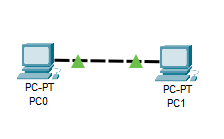
\includegraphics[width=0.5\textwidth]{Conexion cruzada.png}
  \caption{Conexion cruzada entre 2 PCs}
\end{figure}

Para verificar que están conectadas correctamente, podemos configurar la IP de ambas PCs, y utilizar en la Command Prompt el comando ping para probar la conectividad entre PCs.
\begin{figure}[h]
  \centering
  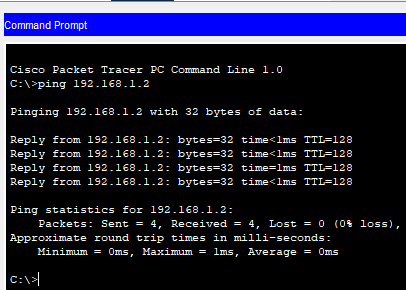
\includegraphics[width=0.5\textwidth]{ping.png}
  \caption{Respuesta del comando ping}
\end{figure}

La limitación principal a esta conexión directa entre 2 PCs es que solo permite conectar dos dispositivos entre sí. Si queremos agregar más dispositivos (como una tercera PC), necesitaríamos un dispositivo adicional como un switch o hub. A su vez, la conexión es única y directa, lo que significa que si el cable o cualquiera de las interfaces falla, la comunicación se interrumpe completamente. No hay redundancia ni mecanismos de recuperación.

\section{Enlaces al material utilizado para realizar el trabajo}
\begin{itemize}
    \item \href{https://www.tokioschool.com/noticias/cisco-packet-tracer/}{https://www.tokioschool.com/noticias/cisco-packet-tracer/}
    \item \href{https://ccnadesdecero.es/que-es-cisco-packet-tracer/}{https://ccnadesdecero.es/que-es-cisco-packet-tracer/}
    \item \href{https://www.ingenieriasystems.com/2016/06/Dispositivos-finales-y-dispositivos-de-red-intermediarios-CCNA1-V5-CISCO-C1.html}{https://www.ingenieriasystems.com/2016/06/Dispositivos-finales-y-dispositivos-de-red-intermediarios-CCNA1-V5-CISCO-C1.html}
    \item \href{https://rodolforodriguezicas.blogspot.com/2017/10/herramientas-de-packet-tracer.html}{https://rodolforodriguezicas.blogspot.com/2017/10/herramientas-de-packet-tracer.html}
    \item \href{http://cidecame.uaeh.edu.mx/lcc/mapa/PROYECTO/libro35/141_estructura_de_la_red.html#:~:text=Algunos%20ejemplos%20de%20dispositivos%20finales,Impresoras%20de%20red}{http://cidecame.uaeh.edu.mx/lcc}
    \item \href{https://cesarcabrera.info/como-usar-packet-tracer-ii-lo-basico/}{https://cesarcabrera.info/como-usar-packet-tracer-ii-lo-basico/}
    \item \href{https://soportedetrabajoscomunicacion.wordpress.com/modulos-de-un-servidor/}{https://soportedetrabajoscomunicacion.wordpress.com/modulos-de-un-servidor/}
    \item \href{https://learningnetwork.cisco.com/s/article/el-software-de-simulacion-cisco-packet-tracer}{https://learningnetwork.cisco.com/s/article/el-software-de-simulacion-cisco-packet-tracer}
    \item \href{https://www.proydesa.org/portal/noticias/1576-hub-switch-y-router-cuales-son-sus-diferencias}{https://www.proydesa.org/portal/noticias/1576-hub-switch-y-router-cuales-son-sus-diferencias}
    \item \href{https://www.cisco.com/c/dam/global/es_mx/assets/ofertas/desconectadosanonimos/routing/pdfs/brochure_redes.pdf}{https://www.cisco.com/c/}
    \item \href{https://www.calameo.com/read/004548756ca708ed116b6}{https://www.calameo.com/read/004548756ca708ed116b6}
    \item \href{https://learningnetwork.cisco.com/s/article/Fundamentos-del-cableado-ethernet-en-una-red-de-datos-empresarial}{https://learningnetwork.cisco.com/Fundamentos-del-cableado-ethernet-en-una-red-de-datos-empresarial}
    \item \href{https://networkips.blogspot.com/2013/03/tipos-de-cables-para-conexiones.html}{https://networkips.blogspot.com/2013/03/tipos-de-cables-para-conexiones.html}
    \item \href{https://todopacketracer.wordpress.com/category/cables/#:~:text=Crossover%20cable%20%2C%20Straight%20cable%2C%20rollover,y%20escuchan%20por%20cable%203.}{https://todopacketracer.wordpress.com/category/cables}
    \item \href{https://estefannyhernandezicas.blogspot.com/2014/10/packet-tracer.html}{https://estefannyhernandezicas.blogspot.com/2014/10/packet-tracer.html}
\end{itemize}

\end{document}
